\section{Introduction}

The Vera C. Rubin Observatory is committed to maintaining the highest standards of security to protect its sensitive data and infrastructure. The Pixel Zone, a designated area within the network of the summit, requires enhanced security measures due to the nature of the data it handles. This document outlines the security protocols and controls implemented to safeguard the Pixel Zone.

\section{Overview of the Pixel Zone}
The Pixel Zone is a critical area within the summit's network infrastructure, responsible for processing and storing high-resolution astronomical data. Given the sensitivity and importance of this data, the Pixel Zone is subject to security controls to prevent unauthorized access and ensure data integrity.

The following is a logic representation of the Pixel zone. 

\begin{figure}
    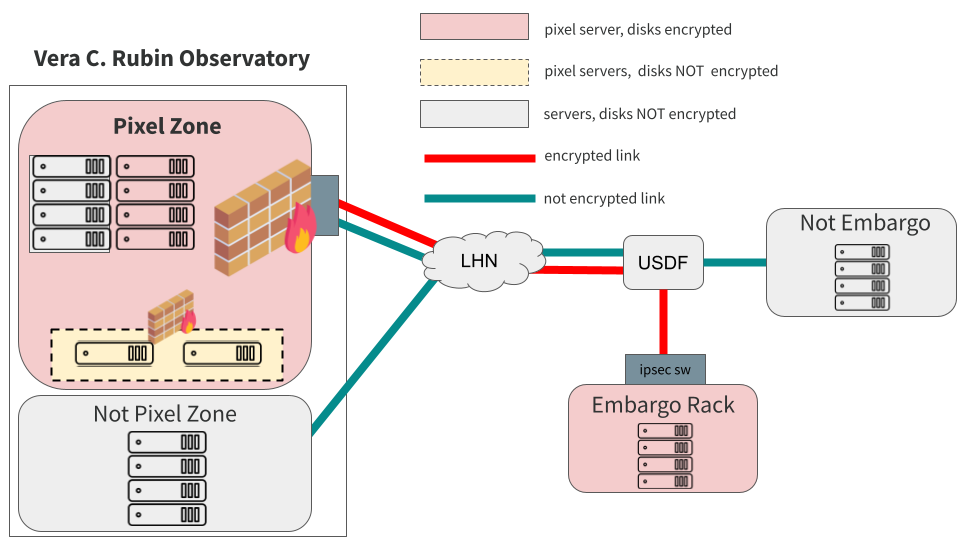
\includegraphics[width=13cm]{emgargo_diagram.png}
    \centering
    \caption*{Logical Topology of Pixel Zone}
  \end{figure}

The Pixel Zone is isolated from users's traffic network at the summit. Users needing to consume services located inside the Pixel Zone will need to open a VPN connection against the concentrator of the Pixel Zone. 

The details of the technical implementation can be reviewed in the document \href{http://ittn-075.lsst.io}{"Rubin Pixel Zone"}


\section{Security Controls}
Strict access control measures are enforced within the Pixel Zone.
\subsection{Physical Controls}
\begin{itemize}
    \item Keyless Access: The entrance of the Summit and Base computer rooms have keyless access control. The administration and audit of the Base computer room is done by NoirLab, but the Summit is done by Rubin Observatory.
    \item Rack Locks: All racks have code based locks (front and rear). The code is unique for each rack and stored in Rubin's password manager, hence its access is controlled and audited.
    \item Sensors: Racks have several environmental sensors, to control temperature, humidity, waterleaks, and also to detect door openings.
    \item CCTV: There's a large deployment of cameras at the summit. The computer rooms cameras record 24/7 and also alert on movements. 
\end{itemize}

The details of the technical implementation can be reviewed in the document \href{http://ittn-077.lsst.io}{"Physical Access Controls"}

\subsection{Logical Controls}
\begin{itemize}
    \item Authentication: Managed by a distributed system as described in \href{http://ittn-010.lsst.io}{User Identification and Authorization}. Users are required to use passwords with a complexity of several factors and history is kept to not repeat passwords. 
    \item Role-Based Access Control (RBAC): Access to resources within the Pixel Zone is granted based on the principle of least privilege. Users are given access only to the information and resources necessary for their roles.
    \item Virtual Private Network (VPN): Internal and External users are required to use a VPN to enter the Pixel Zone. 
    \item Second Factor Authentication: Access to VPN and several services inside the Pixel Zone require 2FA. 
\end{itemize}

\subsection{Encryption at rest and in transit}
To protect data at rest and in transit, the following encryption measures are implemented:

\begin{itemize}
    \item Operating System Encryption: Devices storing pixels within the Pixel Zone are encrypted at operating system level. This ensure confidentiality of the data even if the entire server is stolen.
    \item Storage Encryption: The storage backend (Ceph) where the pixels will be stored, is also encrypted preventing individual disks theft.
    \item Data Transmission Encryption: Data transmitted between Summit and USDF is encrypted via IPSec tunnels, ensuring protection against unauthorized interception and access throughout the data transfer process. The details of the technical implementation can be reviewed in the document \href{http://ittn-076.lsst.io}{"Rubin IPSec Tunnels"}
\end{itemize}

\subsection{Audit and Monitoring}

\begin{itemize}
    \item Audit: Access and critical activities within the Pixel Zone are logged and alerts are triggered when certain conditions are met.
    \item Monitoring: The Pixel Zone is monitored by the Summit observability cluster, hence logs and several metrics are collected and stored for 2+ years.
    \item Alerting: All alerts are managed by Squadcast, which triggers several actions like Slack messages, SMS, Phone calls, etc. 
    
\end{itemize}

\subsection{Network Segmentation}
The Pixel Zone is isolated from other parts of the observatory's network to minimize the risk of unauthorized access and lateral movement of threats:

\begin{itemize}
    \item Firewall Protection: Firewalls are configured to monitor and control incoming and outgoing network traffic to and from the Pixel Zone.
    \item VLAN Isolation: Pixel Zone is isolated from Users' traffic at the summit, including VoIP, Printers, etc.
\end{itemize}

\section{Training and Awareness}
To ensure compliance with security protocols, regular training and awareness programs are conducted for the Chile DevOps team. 

The team engages in the following activities

\begin{itemize}
    \item Conferences.
    \item Purple Team Excercises.
    \item Customized Trainings.
    \item Other activities organized internally.
\end{itemize}
